\chapter{Queueing Models}

\section{Introduction to Queueing Models}
\begin{wrapfigure}{r}{0.4\textwidth}
    \centering
    \vspace{-10pt}
    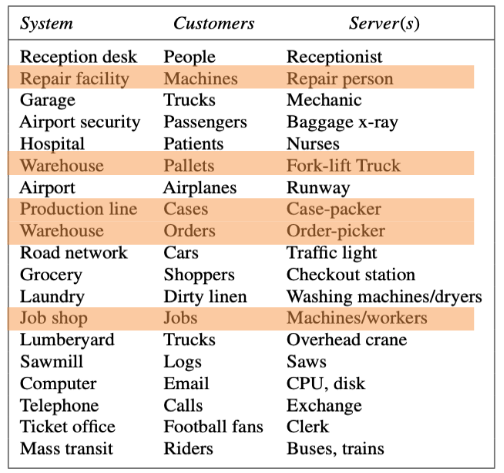
\includegraphics[width=\linewidth]{images/QQ3.png}
    \label{fig:TDlambda}
    \vspace{-10pt}
\end{wrapfigure}
I \textbf{queueing models} sono modelli matematici e di simulazione utilizzati per descrivere e analizzare sistemi in cui delle entità arrivano nel tempo, richiedono un servizio, eventualmente attendono in una coda e, una volta servite, lasciano il sistema.

In questi modelli, il termine \emph{customer} è usato in senso molto generale e non si riferisce necessariamente a una persona. Un customer rappresenta qualsiasi tipo di entità che richiede un servizio a un sistema. Esempi tipici includono prodotti in un sistema di produzione, macchinari che richiedono manutenzione, pacchetti in una rete di comunicazione, veicoli in un sistema di trasporto o materiali in sistemi di movimentazione.

Il comportamento di base di un sistema a coda può essere riassunto attraverso tre fasi fondamentali:
\begin{compactitemize}
    \item i clienti arrivano al sistema nel tempo;
    \item se il servizio non è immediatamente disponibile, si mettono in attesa in una coda;
    \item dopo essere stati serviti, lasciano il sistema.
\end{compactitemize}

I modelli di coda trovano applicazione in numerosi contesti dell’operations management e della supply chain, tra cui sistemi produttivi, impianti di manutenzione, sistemi di comunicazione, reti di trasporto e sistemi di handling dei materiali. In tutti questi ambiti, la presenza di variabilità negli arrivi e nei tempi di servizio rende il comportamento del sistema non banale da analizzare.

I queueing models possono essere studiati seguendo due approcci principali. In alcuni casi, è possibile ottenere risultati tramite metodi matematici e analitici, basati sulla teoria delle probabilità e sui processi stocastici. Tuttavia, tali soluzioni esistono solo per classi limitate di modelli, spesso caratterizzate da ipotesi fortemente restrittive.

In alternativa, i sistemi a coda possono essere analizzati tramite \textbf{simulazione}, che consente di studiare modelli più generali e realistici, superando i limiti dell’analisi puramente matematica. In entrambi i casi, l’obiettivo è quello di predire e comprendere le prestazioni del sistema in funzione dei parametri di input.

Le principali misure di performance tipicamente considerate nei queueing models includono:
\begin{compactitemize}
    \item l’utilization dei server;
    \item la lunghezza delle code;
    \item i ritardi subiti dai clienti.
\end{compactitemize}

Queste misure dipendono da diversi parametri di input, tra cui il tasso di arrivo dei clienti, il tasso di servizio dei server e il numero e la disposizione delle risorse di servizio. L’analisi, matematica o tramite simulazione, permette di valutare come varia il comportamento del sistema al variare di tali parametri, supportando decisioni di progettazione, dimensionamento e gestione operativa.

\subsection{Calling Population}
\begin{wrapfigure}{r}{0.5\textwidth}
    \centering
    \vspace{-10pt}
    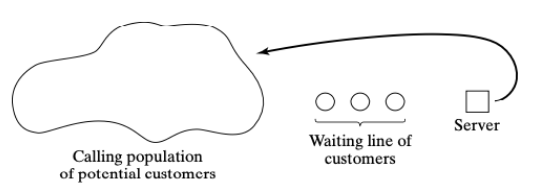
\includegraphics[width=\linewidth]{images/QQ4.png}
    \label{fig:TDlambda}
    \vspace{-10pt}
\end{wrapfigure}
Nei modelli di coda, l’insieme dei potenziali clienti che possono richiedere il servizio a un sistema è detto \textbf{calling population}. Essa rappresenta la sorgente da cui originano gli arrivi al sistema ed è un elemento fondamentale nella modellazione dei processi di arrivo.

La calling population può essere assunta \textbf{finita} oppure \textbf{infinita}, a seconda delle caratteristiche del sistema in esame e degli obiettivi dello studio. Nei sistemi in cui il numero di potenziali clienti è molto elevato, è pratica comune assumere una calling population infinita. Questa assunzione è appropriata quando il numero di clienti presenti nel sistema in un dato istante rappresenta solo una piccola frazione della popolazione totale di potenziali clienti.

Nel caso di \textbf{calling population infinita}, il tasso di arrivo dei clienti è indipendente dal numero di clienti che si trovano attualmente nel sistema o che hanno già lasciato la popolazione. In altre parole, il processo di arrivo non è influenzato dallo stato del sistema: anche se molti clienti sono in coda o in servizio, la probabilità di nuovi arrivi rimane invariata. Questa è l’ipotesi più comune nei modelli classici di teoria delle code.

Al contrario, nei modelli con \textbf{calling population finita}, il tasso di arrivo dipende dal numero di clienti che si trovano nel sistema. Quando alcuni clienti entrano in servizio o sono in attesa, essi vengono temporaneamente rimossi dalla popolazione dei potenziali chiamanti. Di conseguenza, il numero di entità che possono generare nuovi arrivi diminuisce e il tasso di arrivo si riduce.

Un esempio tipico di calling population finita è rappresentato da un reparto ospedaliero con un numero limitato di pazienti assegnati a una singola infermiera. Quando tutti i pazienti sono a riposo e nessuno richiede assistenza, l’infermiera è idle e il tasso di arrivo delle richieste è massimo. Man mano che i pazienti iniziano a richiedere assistenza e a entrare in attesa o in servizio, la popolazione dei potenziali chiamanti si riduce. Quando tutti i pazienti sono in attesa o in servizio, non vi sono più pazienti disponibili a generare nuove richieste, e il tasso di arrivo diventa pari a zero.

La distinzione tra calling population finita e infinita è cruciale nella costruzione di un modello di coda, poiché influisce direttamente sulla struttura del processo di arrivo e, di conseguenza, sul comportamento complessivo del sistema.

\subsection{System Capacity}

In molti queueing models esiste un limite al numero di clienti che possono essere presenti nel sistema o nella coda di attesa in un determinato istante. Questo limite è indicato come \textbf{system capacity} e può essere imposto per ragioni fisiche, operative o di policy.

La system capacity può riferirsi alla sola coda di attesa oppure all’intero sistema, comprendendo sia i clienti in servizio sia quelli in attesa. Quando il numero massimo consentito di clienti nel sistema viene raggiunto, si dice che il sistema è \emph{full}.

In presenza di una capacità finita, un cliente che arriva e trova il sistema pieno non entra nel sistema stesso, ma viene immediatamente respinto e ritorna alla calling population. Questo comportamento è tipico, ad esempio, di sistemi con spazio limitato, come sale d’attesa di dimensione finita o sistemi informatici con un numero massimo di richieste simultanee gestibili.

L’introduzione di una capacità finita rende necessario distinguere tra due diversi concetti di tasso di arrivo. Il primo è l’\textbf{arrival rate}, che rappresenta il numero di clienti che tentano di entrare nel sistema per unità di tempo. Il secondo è l’\textbf{effective arrival rate}, che indica il numero di clienti che riescono effettivamente a entrare nel sistema per unità di tempo.

Quando il sistema non è mai pieno, i due tassi coincidono. Tuttavia, in presenza di una capacità limitata, una parte dei clienti in arrivo può essere rifiutata, determinando una differenza tra arrival rate ed effective arrival rate. Questa distinzione è fondamentale per una corretta valutazione delle prestazioni del sistema, poiché molte misure di performance dipendono dal flusso effettivo di clienti che entrano nel sistema, piuttosto che dal numero totale di tentativi di arrivo.

La considerazione della system capacity introduce quindi un ulteriore livello di realismo nei modelli di coda e ha un impatto diretto sulle dinamiche di congestione e sulle prestazioni complessive del sistema.

\subsection{Arrival Process (Infinite Population Case)}

Nei queueing models con calling population infinita, il processo di arrivo dei clienti è generalmente descritto in termini dei \textbf{tempi di interarrivo} tra clienti successivi. In questo contesto, l’evoluzione degli arrivi non è influenzata dallo stato del sistema, poiché la popolazione di potenziali clienti è considerata sufficientemente grande.

Gli arrivi possono avvenire in modi differenti. In alcuni sistemi, i clienti arrivano a \textbf{tempi programmati}, come nel caso di appuntamenti o schedulazioni prestabilite. In molti altri contesti, invece, gli arrivi avvengono a \textbf{tempi casuali}. In questo caso, il processo di arrivo viene descritto tramite una distribuzione di probabilità che modella l’incertezza associata ai tempi di interarrivo.

Gli arrivi possono inoltre avvenire:
\begin{compactitemize}
    \item uno alla volta;
    \item in \textbf{batch}, ovvero gruppi di clienti che arrivano simultaneamente.
\end{compactitemize}

Nel caso di arrivi a batch, la dimensione del gruppo può essere costante oppure casuale, a seconda del sistema modellato. Questa caratteristica ha un impatto significativo sulla dinamica delle code e deve essere esplicitamente considerata nella costruzione del modello.

Il modello più importante e più comunemente utilizzato per descrivere arrivi casuali nei sistemi a coda è il \textbf{Poisson arrival process}. Sia $A_n$ il tempo di interarrivo tra il cliente $n-1$ e il cliente $n$. Nel processo di Poisson, i tempi di interarrivo $A_n$ sono variabili casuali indipendenti ed esponenzialmente distribuite con media $1/\lambda$, dove $\lambda$ rappresenta il \textbf{tasso di arrivo}, espresso come numero medio di clienti per unità di tempo.

Una proprietà fondamentale del processo di Poisson è che il numero di arrivi in un intervallo di tempo di ampiezza $\Delta t$ segue una distribuzione di Poisson con valore atteso pari a $\lambda \cdot \Delta t$. Questa caratteristica rende il processo di Poisson particolarmente adatto a modellare sistemi in cui gli arrivi avvengono in modo casuale e indipendente nel tempo.

I processi di arrivo Poisson sono tipicamente utilizzati per descrivere sistemi con una grande calling population, in cui ciascun cliente prende decisioni indipendenti su quando richiedere il servizio. Per questo motivo, il processo di Poisson rappresenta un punto di riferimento fondamentale sia nei modelli analitici di teoria delle code sia negli studi di simulazione a eventi discreti.

\subsection{Arrival Process (Finite Population Case)}

Nei queueing models con \textbf{calling population finita}, il processo di arrivo dei clienti presenta caratteristiche diverse rispetto al caso di popolazione infinita, poiché il numero di potenziali clienti che possono richiedere il servizio è limitato.

Un cliente è detto \textbf{pending} quando appartiene alla calling population, ossia quando non si trova né in servizio né in attesa nel sistema. Dopo aver lasciato il sistema, il cliente ritorna nella calling population e rimane in tale stato per un certo periodo di tempo prima di generare una nuova richiesta di servizio.

Il tempo che intercorre tra la partenza di un cliente dal sistema e il suo successivo arrivo è chiamato \textbf{runtime}. Indicando con $A_1^{(i)}, A_2^{(i)}, \dots$ i runtime successivi del cliente $i$, questi rappresentano le realizzazioni del processo di arrivo per ciascuna entità della popolazione finita.

Ad ogni runtime corrisponde un tempo di servizio e un tempo di attesa in coda. In particolare, si indicano con $S_1^{(i)}, S_2^{(i)}, \dots$ i tempi di servizio associati ai successivi accessi del cliente $i$ al sistema, e con $W_{Q,1}^{(i)}, W_{Q,2}^{(i)}, \dots$ i corrispondenti tempi di attesa in coda.

Il tempo totale trascorso nel sistema dal cliente $i$ durante la sua $n$-esima visita è quindi dato dalla somma del tempo di attesa in coda e del tempo di servizio:
\[
W_n^{(i)} = W_{Q,n}^{(i)} + S_n^{(i)}
\]

I modelli a popolazione finita trovano un’importante applicazione pratica nel cosiddetto \textbf{machine-repair problem}. In questo contesto, i clienti sono rappresentati da macchine che, dopo un certo periodo di funzionamento, si guastano e richiedono un intervento di riparazione. I runtime corrispondono quindi ai \emph{time-to-failure}, ossia ai tempi di funzionamento delle macchine tra due guasti consecutivi.

I time-to-failure sono comunemente modellati tramite distribuzioni di probabilità continue come l’esponenziale, la Weibull o la gamma. In molti modelli si assume che i tempi di guasto successivi siano indipendenti tra loro. Tuttavia, in applicazioni più realistiche, tali tempi possono dipendere da fattori aggiuntivi, come l’età o lo stato di usura della macchina.

Il caso di popolazione finita richiede quindi una descrizione più articolata del processo di arrivo, poiché il tasso di arrivo complessivo del sistema dipende direttamente dal numero di entità attualmente presenti nella calling population.

\subsection{Queue Behaviour and Queue Discipline}

Il \textbf{queue behaviour} descrive il comportamento dei clienti mentre si trovano in coda o nel sistema. In molti modelli di coda, in particolare quelli più semplici, si assume implicitamente che i clienti attendano pazientemente fino a quando non vengono serviti. Tuttavia, in numerose applicazioni reali, i clienti possono reagire allo stato della coda adottando comportamenti differenti.

Un primo comportamento possibile è il \textbf{balking}. Un cliente balks quando, al momento dell’arrivo, osserva una coda e decide di non entrare nel sistema perché la lunghezza della coda è ritenuta eccessiva. In questo caso, il cliente lascia immediatamente il sistema senza ricevere servizio.

Un secondo comportamento è il \textbf{reneging}. Un cliente reneges se entra nel sistema ma decide di abbandonare la coda dopo aver atteso per un certo periodo di tempo, senza essere stato servito. Questo comportamento è spesso modellato introducendo una variabile casuale che rappresenta la tolleranza massima all’attesa di ciascun cliente.

Un ulteriore comportamento è il \textbf{jockeying}, che si verifica nei sistemi con più code parallele. In questo caso, un cliente può decidere di spostarsi da una coda a un’altra, nella percezione che quest’ultima possa garantire un servizio più rapido.

Accanto al comportamento dei clienti, un ruolo centrale nella definizione di un sistema a coda è svolto dalla \textbf{queue discipline}. La queue discipline definisce l’ordine logico secondo il quale i clienti in attesa vengono selezionati per ricevere il servizio e determina quindi quale cliente verrà servito per primo.

Le principali discipline di servizio comunemente utilizzate nei queueing models includono:
\begin{compactitemize}
    \item \textbf{First-In-First-Out (FIFO)}, in cui i clienti sono serviti nell’ordine di arrivo;
    \item \textbf{Last-In-First-Out (LIFO)}, in cui l’ultimo cliente arrivato è il primo a essere servito;
    \item \textbf{Service-In-Random-Order (SIRO)}, in cui il prossimo cliente da servire è scelto in modo casuale tra quelli in coda;
    \item \textbf{Shortest-Processing-Time-First (SPT)}, in cui viene servito per primo il cliente con il tempo di servizio più breve;
    \item \textbf{Priority rules (PR)}, in cui i clienti sono serviti in base a livelli di priorità predefiniti.
\end{compactitemize}

La scelta della queue discipline ha un impatto significativo sulle prestazioni del sistema e sull’esperienza dei clienti. Discipline diverse possono portare a differenze sostanziali nei tempi di attesa medi, nella variabilità dei ritardi e nella percezione di equità del servizio. Per questo motivo, la modellazione del comportamento dei clienti e della disciplina di servizio rappresenta un aspetto cruciale nella costruzione di modelli di coda realistici ed efficaci.

\subsection{Service Times and the Service Mechanism}

Nei queueing models, il \textbf{service time} rappresenta la durata del tempo necessario a un server per completare il servizio di un cliente. Siano $S_1, S_2, S_3, \dots$ i tempi di servizio associati agli arrivi successivi al sistema. I service times costituiscono una componente fondamentale del modello, poiché influenzano direttamente le prestazioni complessive del sistema.

I tempi di servizio possono essere \textbf{costanti} oppure \textbf{casuali}. Nel primo caso, ogni cliente richiede la stessa quantità di tempo per essere servito. Nel secondo caso, la durata del servizio è modellata come una variabile casuale. Le distribuzioni di probabilità più comunemente utilizzate per descrivere service times casuali includono la distribuzione esponenziale, Weibull, gamma, lognormale e normale troncata.

In alcuni sistemi, i tempi di servizio non sono uguali per tutti i clienti, ma dipendono dal tipo di cliente o dalla classe di servizio. In questi casi, si utilizzano distribuzioni diverse per rappresentare i service times associati a ciascuna tipologia di cliente, introducendo un ulteriore livello di dettaglio e realismo nel modello.

Un sistema di coda può essere visto come una rete composta da uno o più \textbf{service centers} e dalle relative code che li connettono. Ogni service center è costituito da un certo numero di server che operano in parallelo.

Una configurazione comune è quella con una \textbf{singola coda} davanti a un insieme di server paralleli. In questo caso, i clienti attendono in un’unica linea e, non appena un server si libera, il prossimo cliente in coda viene assegnato al primo server disponibile.

A seconda del numero di server che operano in parallelo, i service mechanisms possono essere classificati come segue:
\begin{compactitemize}
    \item \textbf{Single-server}, con un solo server ($c = 1$);
    \item \textbf{Multi-server}, con un numero finito di server in parallelo ($1 < c < \infty$);
    \item \textbf{Unlimited servers}, con un numero teoricamente infinito di server ($c = \infty$), come nei sistemi di self-service.
\end{compactitemize}

La scelta del meccanismo di servizio e della distribuzione dei tempi di servizio ha un impatto significativo sulle prestazioni del sistema, influenzando l’utilization dei server, la lunghezza delle code e i ritardi sperimentati dai clienti. Per questo motivo, una corretta modellazione dei service times e del service mechanism è essenziale nella costruzione di queueing models affidabili.

\subsection{Queueing Notation}
\begin{wrapfigure}{r}{0.4\textwidth}
    \centering
    \vspace{-10pt}
    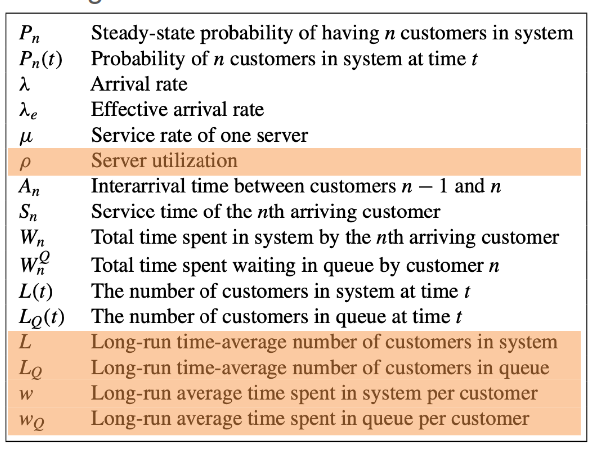
\includegraphics[width=\linewidth]{images/QQ5.png}
    \label{fig:TDlambda}
    \vspace{-10pt}
\end{wrapfigure}
Per descrivere in modo compatto e standardizzato i queueing models, viene comunemente utilizzato un sistema di notazione noto come \textbf{notazione di Kendall}. Questa notazione consente di rappresentare le caratteristiche fondamentali di un sistema a coda attraverso una forma simbolica sintetica.

La notazione standard di Kendall è espressa come:
\[
A / B / c / N / K
\]
dove ciascun simbolo rappresenta una specifica componente del sistema.

Il simbolo $A$ indica la distribuzione dei tempi di interarrivo dei clienti.  
Il simbolo $B$ rappresenta la distribuzione dei tempi di servizio.  
Il parametro $c$ denota il numero di server che operano in parallelo nel sistema.  
Il parametro $N$ rappresenta la capacità massima del sistema, ovvero il numero massimo di clienti che possono essere presenti contemporaneamente nel sistema, includendo sia quelli in attesa sia quelli in servizio.  
Infine, il parametro $K$ indica la dimensione della calling population.

Nel caso in cui alcuni parametri non siano specificati, si assumono valori di default. In particolare, se $N$ o $K$ non sono indicati, essi vengono generalmente considerati infiniti.

Per i simboli $A$ e $B$, che descrivono i processi di arrivo e di servizio, vengono utilizzate alcune notazioni standard:
\begin{compactitemize}
    \item \textbf{M} (Markov), che indica tempi esponenzialmente distribuiti;
    \item \textbf{D} (Deterministic), per tempi costanti;
    \item \textbf{$E_k$} (Erlang di ordine $k$);
    \item \textbf{G} (General), per una distribuzione arbitraria;
    \item \textbf{GI} (General Independent), per distribuzioni generiche con osservazioni indipendenti.
\end{compactitemize}

Questa notazione permette di identificare rapidamente le ipotesi strutturali di un modello di coda e di confrontare sistemi diversi in modo immediato.

Come esempio, il modello:
\[
M/M/1/\infty/\infty
\]
descrive un sistema a singolo server con arrivi Poisson, tempi di servizio esponenziali, capacità di coda illimitata e calling population infinita. Questo modello è comunemente indicato in forma abbreviata come:
\[
M/M/1
\]

Un altro esempio tipico è un sistema con una popolazione finita. Ad esempio, una infermiera che assiste cinque pazienti può essere modellata come:
\[
M/M/1/5/5
\]
In questo caso, sia la capacità del sistema sia la calling population sono limitate a cinque clienti.

La notazione di Kendall fornisce quindi un linguaggio comune per descrivere, classificare e analizzare sistemi di coda, risultando fondamentale sia nello studio analitico sia nella simulazione dei queueing models.

\subsection{Time-Average Number in System L}

Una misura di performance di interesse generale nei queueing models è il \textbf{time-average number of customers in system}, indicato con $L$. Questa quantità rappresenta il numero medio di clienti presenti nel sistema nel tempo, includendo sia i clienti in attesa sia quelli in servizio.
\begin{wrapfigure}{r}{0.4\textwidth}
    \centering
    \vspace{-10pt}
    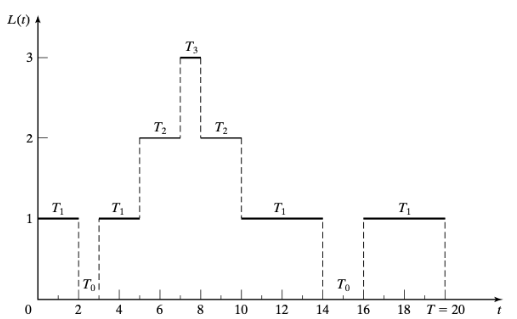
\includegraphics[width=\linewidth]{images/QQ6.png}
    \label{fig:TDlambda}
    \vspace{-10pt}
\end{wrapfigure}
Si consideri un sistema generale descritto dalla notazione $G/G/c/N/K$. Sia $L(t)$ il numero di clienti presenti nel sistema all’istante di tempo $t$. Durante l’evoluzione della simulazione, il processo $L(t)$ assume valori interi non negativi.

Sia $T$ l’orizzonte temporale della simulazione. Indichiamo con $T_i$ il tempo totale, nell’intervallo $[0, T]$, durante il quale il sistema contiene esattamente $i$ clienti. Per definizione, vale che:
\[
\sum_{i=0}^{\infty} T_i = T
\]

Un estimatore naturale del time-average number of customers in system è dato da:
\[
\hat{L} = \frac{1}{T} \sum_{i=0}^{\infty} i \cdot T_i
\]

Questa espressione può essere riscritta in forma equivalente osservando che la somma pesata dei tempi $T_i$ coincide con l’integrale nel tempo del processo $L(t)$. In particolare:
\[
\sum_{i=0}^{\infty} i \cdot T_i = \int_{0}^{T} L(t)\, dt
\]
e quindi:
\[
\hat{L} = \frac{1}{T} \int_{0}^{T} L(t)\, dt
\]

L’estimatore $\hat{L}$ rappresenta una \textbf{time-average} ed è un estimatore consistente del valore atteso $L$. In particolare, al crescere della durata della simulazione, vale che:
\[
\hat{L} \longrightarrow L \quad \text{per } T \to \infty
\]
Per questa ragione, l’estimatore $\hat{L}$ è detto \textbf{fortemente consistente} per $L$: se la simulazione viene eseguita per un tempo sufficientemente lungo, la stima ottenuta diventa arbitrariamente vicina al valore atteso reale.

Tuttavia, per valori finiti di $T$, la stima $\hat{L}$ dipende dalle \textbf{condizioni iniziali} del sistema al tempo $t = 0$. Ad esempio, avviare la simulazione in uno stato vuoto può introdurre un bias nelle stime iniziali. Questo aspetto rende necessario, in molte applicazioni, considerare un periodo di warm-up prima di raccogliere osservazioni utilizzabili per l’analisi delle prestazioni.

Il time-average number in system costituisce una misura chiave nelle analisi di simulazione ed è strettamente collegata ad altre grandezze fondamentali, come il delay medio e la queue size media, attraverso relazioni teoriche quali la Little’s Law.

\subsection{Time-Average Number in Queue $L_Q$}

Un’ulteriore misura di performance di grande importanza nei queueing models è il \textbf{time-average number of customers in queue}, indicato con $L_Q$. Questa quantità rappresenta il numero medio di clienti in attesa nella coda, calcolato come media nel tempo.

Analogamente al caso del numero medio nel sistema, la stima di $L_Q$ si basa sull’osservazione dell’evoluzione temporale della lunghezza della coda. Sia $L_Q(t)$ il numero di clienti presenti in coda all’istante di tempo $t$. Durante la simulazione, $L_Q(t)$ assume valori interi non negativi.

Sia $T$ la durata totale della simulazione e indichiamo con $T_i^Q$ il tempo complessivo, nell’intervallo $[0, T]$, durante il quale la coda contiene esattamente $i$ clienti. Un estimatore naturale del time-average number in queue è definito come:
\[
\hat{L}_Q = \frac{1}{T} \sum_{i=0}^{\infty} i \cdot T_i^Q
\]

In modo equivalente, tale stimatore può essere espresso come media nel tempo del processo $L_Q(t)$:
\[
\hat{L}_Q = \frac{1}{T} \int_{0}^{T} L_Q(t)\, dt
\]

L’estimatore $\hat{L}_Q$ è consistente per il valore atteso $L_Q$. In particolare, se la durata della simulazione cresce indefinitamente, vale che:
\[
\hat{L}_Q \longrightarrow L_Q \quad \text{per } T \to \infty
\]

Per definizione, il numero di clienti in coda può essere espresso in funzione del numero totale di clienti nel sistema. In particolare:
\[
L_Q(t) =
\begin{cases}
0 & \text{se } L(t) = 0, \\
L(t) - 1 & \text{se } L(t) \geq 1,
\end{cases}
\]
ossia, quando il sistema è vuoto non esiste alcuna coda, mentre quando il sistema contiene almeno un cliente, uno di essi è in servizio e i restanti costituiscono la coda.

Come per le altre misure time-average, anche la stima di $L_Q$ dipende dalle condizioni iniziali per valori finiti di $T$. Di conseguenza, un’adeguata gestione del periodo di warm-up è essenziale per ottenere stime affidabili della lunghezza media della coda.

\subsection{Average Time Spent in System and in Queue}

Un’ulteriore classe di misure di performance di grande interesse nei queueing models riguarda il \textbf{tempo medio trascorso dai clienti nel sistema} e il \textbf{tempo medio trascorso in coda}. Queste grandezze descrivono l’esperienza dei clienti e sono quindi misure di performance dal punto di vista dell’utente del sistema.

Sia $W_i$ il tempo totale trascorso nel sistema dal cliente $i$, comprensivo sia del tempo di attesa in coda sia del tempo di servizio. Il tempo medio trascorso nel sistema può essere stimato tramite la media dei tempi osservati sui primi $N$ clienti:
\[
\hat{w} = \frac{1}{N} \sum_{i=1}^{N} W_i
\]

Analogamente, indicando con $W_{Q,i}$ il tempo trascorso in coda dal cliente $i$, il tempo medio di attesa in coda è stimato da:
\[
\hat{w}_Q = \frac{1}{N} \sum_{i=1}^{N} W_{Q,i}
\]

Al crescere del numero di clienti osservati, tali stimatori convergono ai rispettivi valori attesi:
\[
\hat{w} \longrightarrow w \quad \text{per } N \to \infty
\]
\[
\hat{w}_Q \longrightarrow w_Q \quad \text{per } N \to \infty
\]

Le quantità $w$ e $w_Q$ rappresentano rispettivamente l’average time spent in system e l’average time spent in queue.

Analogamente a quanto avviene per le misure time-average come $\hat{L}$ e $\hat{L}_Q$, anche gli stimatori $\hat{w}$ e $\hat{w}_Q$ sono influenzati dalle \textbf{condizioni iniziali} del sistema al tempo $t = 0$ e dalla durata complessiva della simulazione. In particolare, per valori finiti di $N$ e di $T$, le stime ottenute possono essere affette da bias transitori.

Per questo motivo, nella pratica della simulazione è spesso necessario introdurre un periodo di warm-up e osservare un numero sufficientemente elevato di clienti, al fine di ottenere stime affidabili e rappresentative delle reali prestazioni del sistema.

\subsection{Conservation Equation (Little’s Law)}

Una relazione fondamentale nei queueing models è la cosiddetta \textbf{conservation equation}, più comunemente nota come \textbf{Little’s Law}. Questa relazione collega in modo semplice ed estremamente generale alcune delle principali misure di performance di un sistema a coda.

Sia $\lambda$ il tasso medio di arrivo dei clienti nel lungo periodo. Durante una simulazione di durata $T$, sia $N$ il numero totale di clienti che arrivano al sistema. Un estimatore naturale del tasso di arrivo è dato da:
\[
\hat{\lambda} = \frac{N}{T}
\]
Al crescere del numero di osservazioni e della durata della simulazione, tale estimatore converge al vero valore del tasso di arrivo:
\[
\hat{\lambda} \longrightarrow \lambda \quad \text{per } N, T \to \infty
\]

Indicando con $\hat{L}$ il numero medio di clienti nel sistema calcolato come media nel tempo, e con $\hat{w}$ il tempo medio trascorso nel sistema calcolato come media sui clienti, vale la seguente relazione asintotica:
\[
\hat{L} = \hat{\lambda} \cdot \hat{w}
\]
e, nel limite,
\[
L = \lambda \cdot w \quad \text{per } N, T \to \infty
\]

Questa equazione afferma che il numero medio di clienti presenti nel sistema in un istante arbitrario è uguale al prodotto tra il tasso medio di arrivo e il tempo medio che un cliente trascorre nel sistema. Tale risultato è noto come \textbf{Little’s Law} e rappresenta una delle relazioni più importanti e più generali nella teoria delle code.

Un aspetto cruciale della Little’s Law è la sua \emph{notevole generalità}. La relazione vale indipendentemente dalla distribuzione dei tempi di interarrivo e di servizio, dalla disciplina di coda, dal numero di server o dalla presenza di capacità finite, purché il sistema sia stabile e osservato nel lungo periodo.

Un modo informale di derivare la relazione $\hat{L} = \hat{\lambda} \cdot \hat{w}$ consiste nell’osservare che la somma dei tempi trascorsi nel sistema da tutti i clienti può essere espressa in due modi equivalenti. Da un lato, essa è pari alla somma dei tempi individuali:
\[
\sum_{i=1}^{N} W_i
\]
Dall’altro lato, la stessa quantità corrisponde all’integrale nel tempo del numero di clienti presenti nel sistema:
\[
\int_{0}^{T} L(t)\, dt
\]

Uguagliando le due espressioni e dividendo per $T$, si ottiene:
\[
\hat{L} = \frac{1}{T} \int_{0}^{T} L(t)\, dt
         = \frac{N}{T} \cdot \frac{1}{N} \sum_{i=1}^{N} W_i
         = \hat{\lambda} \cdot \hat{w}
\]

Nel limite del lungo periodo, questa relazione converge alla forma teorica della Little’s Law. La conservation equation fornisce quindi un potente strumento di verifica e interpretazione dei risultati di simulazione, permettendo di controllare la coerenza delle stime ottenute per le diverse misure di performance.

\subsection{Server Utilization}
\begin{wrapfigure}{r}{0.4\textwidth}
    \centering
    \vspace{-10pt}
    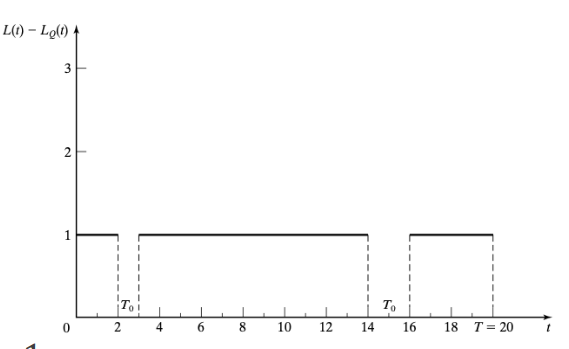
\includegraphics[width=\linewidth]{images/QQ7.png}
    \label{fig:TDlambda}
    \vspace{-10pt}
\end{wrapfigure}
Una misura di performance centrale nei queueing models è la \textbf{server utilization}, indicata con $\rho$. Questa grandezza rappresenta la proporzione di tempo, nel lungo periodo, durante la quale il server è occupato.

Dal punto di vista simulativo, l’utilizzation del server può essere stimata come media nel tempo dello stato del server. Indicando con $\hat{\rho}$ l’estimatore dell’utilization, vale che:
\[
\hat{\rho} \longrightarrow \rho \quad \text{per } T \to \infty
\]

Si consideri innanzitutto il caso di una coda a singolo server del tipo $G/G/1$, con tasso medio di arrivo pari a $\lambda$ clienti per unità di tempo e tempo medio di servizio pari a $E[S] = 1/\mu$. Quando il server è attivo, esso opera quindi con tasso di servizio $\mu$.

Applicando la Little’s Law al sottosistema del server, si osserva che il tempo medio trascorso nel servizio è pari al tempo medio di servizio, ossia:
\[
w = E[S] = \frac{1}{\mu}
\]

Il numero medio di clienti nel sottosistema del server è dato dalla media nel tempo della variabile indicatrice che vale 1 quando il server è busy e 0 quando è idle. Tale quantità coincide con la frazione di tempo in cui il server è occupato, cioè con l’utilization. Formalmente:
\[
\hat{L}_S = \frac{1}{T} \int_{0}^{T} \bigl(L(t) - L_Q(t)\bigr)\, dt = \frac{T - T_0}{T} = \hat{\rho}
\]
dove $T_0$ rappresenta il tempo complessivo in cui il sistema è vuoto.

Combinando queste osservazioni, si ottiene la relazione fondamentale per il server utilization:
\[
\rho = \lambda E[S] = \frac{\lambda}{\mu}
\]

Affinché un sistema $G/G/1$ sia stabile, è necessario che il tasso di arrivo sia inferiore al tasso di servizio, ovvero:
\[
\lambda < \mu \quad \text{oppure} \quad \rho < 1
\]

Se questa condizione non è soddisfatta e $\lambda > \mu$, il server non è in grado di smaltire i clienti con sufficiente rapidità. In tal caso, la coda cresce nel tempo con un tasso medio pari a $(\lambda - \mu)$ clienti per unità di tempo e le misure di performance non ammettono valori stazionari ben definiti.

Nel caso più generale di una coda $G/G/c$ con $c$ server in parallelo, ciascun server ha tempo medio di servizio pari a $1/\mu$ e il tasso di servizio complessivo del sistema è pari a $c\mu$. Il numero medio di server occupati nel lungo periodo è dato da:
\[
L_S = \lambda E[S] = \frac{\lambda}{\mu}
\]

La server utilization media è quindi pari a:
\[
\rho = \frac{L_S}{c} = \frac{\lambda}{c\mu}
\]

Affinché il sistema sia stabile, è necessario che il tasso di arrivo sia inferiore alla capacità complessiva di servizio, ossia:
\[
\lambda < c\mu
\]

La server utilization costituisce quindi un indicatore chiave per valutare sia la stabilità sia il livello di saturazione di un sistema a coda, ed è spesso utilizzata per identificare colli di bottiglia e supportare decisioni di dimensionamento delle risorse.

\subsection{Exercise 1: Bank with Multiple Clerks}

Si consideri una banca in cui i clienti arrivano in modo casuale con un tasso medio di arrivo pari a $\lambda = 50$ clienti per ora. Il sistema è dotato di $c = 20$ sportelli (clerks), ciascuno dei quali è in grado di servire clienti con un tasso medio di servizio pari a $\mu = 5$ clienti per ora.

Il sistema può essere modellato come una coda $G/G/20$ con calling population infinita. Il tasso di servizio complessivo del sistema è pari a $c\mu = 100$ clienti per ora. La server utilization media è quindi:
\[
\rho = \frac{\lambda}{c\mu} = \frac{50}{20 \cdot 5} = 0.5
\]

Questo valore indica che, nel lungo periodo, ciascun server è occupato mediamente per il $50\%$ del tempo. Il numero medio di server occupati è dato da:
\[
L_S = \frac{\lambda}{\mu} = \frac{50}{5} = 10
\]
ossia, in media, 10 sportelli risultano occupati contemporaneamente.

Affinché il sistema sia stabile, è necessario che il numero di server soddisfi la condizione:
\[
c > \frac{\lambda}{\mu}
\]
In questo caso, poiché $c = 20 > 10$, il sistema è chiaramente stabile.

Sebbene la stabilità e il livello medio di utilizzo dei server possano essere facilmente determinati, la valutazione dei ritardi dei clienti e della lunghezza della coda risulta meno immediata. In particolare, anche in presenza di un utilization relativamente basso, la variabilità nei tempi di arrivo e di servizio può generare attese non trascurabili. La stima dei customer delays e della lunghezza media della coda richiede quindi un’analisi più approfondita, basata su modelli analitici specifici o su simulazione.

\subsection{Exercise 2: Scheduled Physician Appointments}

Si consideri un medico che programma gli appuntamenti dei pazienti ogni 10 minuti. Il processo di arrivo è quindi deterministico, mentre i tempi di servizio sono casuali e descritti dalla seguente distribuzione discreta:
\[
S_i =
\begin{cases}
9 \text{ minuti} & \text{con probabilità } 0.9, \\
12 \text{ minuti} & \text{con probabilità } 0.1.
\end{cases}
\]

Il tempo medio di servizio è:
\[
E[S_i] = 9 \cdot 0.9 + 12 \cdot 0.1 = 9.3 \text{ minuti}
\]

Poiché i pazienti arrivano ogni 10 minuti, il tempo medio di interarrivo è $E[A] = 10$ minuti. La server utilization risulta quindi:
\[
\rho = \frac{E[S]}{E[A]} = \frac{9.3}{10} = 0.93
\]
Poiché $\rho < 1$, il sistema risulta stabile.

Tuttavia, la sola condizione di stabilità non è sufficiente a garantire ritardi trascurabili. La varianza dei tempi di servizio è:
\[
\operatorname{Var}(S_i) = E[S_i^2] - (E[S_i])^2 = 0.81 \text{ minuti}^2
\]

La presenza di variabilità nei tempi di servizio implica che, anche con un utilization inferiore a uno, si formeranno inevitabilmente delle code. In particolare, alcuni appuntamenti richiederanno più tempo del previsto, causando ritardi che si propagano ai pazienti successivi.

Questo esercizio mette in evidenza come, nei sistemi di servizio schedulati, una elevata utilization combinata con variabilità nei tempi di servizio possa condurre a code significative. Un confronto tra l’intuizione sul massimo livello di congestione e i risultati ottenuti tramite simulazione permette di comprendere meglio l’impatto della variabilità sul comportamento del sistema.

\subsection{Infinite Population Markovian Models}
\begin{wrapfigure}{r}{0.4\textwidth}
    \centering
    \vspace{-10pt}
    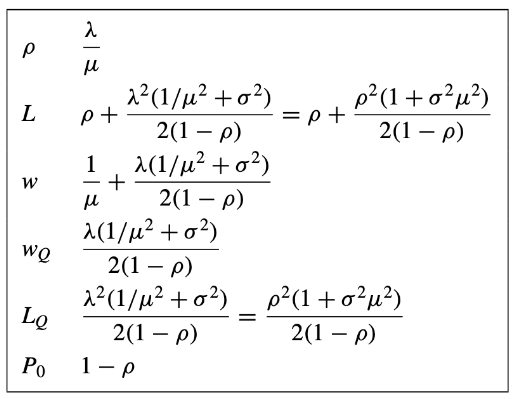
\includegraphics[width=\linewidth]{images/QQ8.png}
    \label{fig:TDlambda}
    \vspace{-10pt}
\end{wrapfigure}
Una classe particolarmente importante di queueing models è rappresentata dai \textbf{modelli markoviani a popolazione infinita}. In questi modelli si assume che la calling population sia infinita e che il processo di arrivo dei clienti segua un \textbf{processo di Poisson} con tasso $\lambda$, espresso come numero medio di arrivi per unità di tempo.

Equivalentemente, i tempi di interarrivo tra clienti successivi sono variabili casuali indipendenti ed esponenzialmente distribuite con valore medio pari a $1/\lambda$. Questa proprietà implica che il processo di arrivo è privo di memoria, caratteristica fondamentale per la trattabilità matematica dei modelli markoviani.

I tempi di servizio possono essere anch’essi esponenzialmente distribuiti, dando luogo a modelli di tipo \textbf{M/M/1}, oppure seguire una distribuzione arbitraria, come nel caso dei modelli \textbf{M/G/1}. In entrambi i casi, si assume che la disciplina di coda sia \textbf{FIFO}.

Un concetto centrale nello studio di questi modelli è quello di \textbf{equilibrio statistico}, o \textbf{steady-state}. Il sistema si dice in steady-state se la distribuzione di probabilità del numero di clienti nel sistema non dipende dal tempo. Formalmente, indicando con $L(t)$ il numero di clienti nel sistema all’istante $t$, vale che:
\[
P\{L(t) = n\} = P_n \quad \text{per ogni } t
\]
dove $P_n$ rappresenta la probabilità stazionaria di trovare $n$ clienti nel sistema.

Il numero medio di clienti nel sistema in steady-state è quindi definito come:
\[
L = \sum_{n=0}^{\infty} n P_n
\]

Una volta noto il valore di $L$, le altre principali misure di performance possono essere derivate direttamente mediante la \textbf{Little’s Law}. In particolare, il tempo medio trascorso nel sistema è dato da:
\[
w = \frac{L}{\lambda}
\]
mentre il tempo medio di attesa in coda è:
\[
w_Q = w - \frac{1}{\mu}
\]
dove $1/\mu$ rappresenta il tempo medio di servizio. Di conseguenza, il numero medio di clienti in attesa in coda è:
\[
L_Q = \lambda w_Q
\]

Un caso di grande rilevanza è il modello \textbf{M/G/1}, in cui i tempi di arrivo sono Poisson e i tempi di servizio seguono una distribuzione generica con media $1/\mu$ e varianza $\sigma^2$. Anche in questo caso, il sistema ammette uno steady-state se e solo se la server utilization soddisfa la condizione:
\[
\rho = \frac{\lambda}{\mu} < 1
\]

Se tale condizione è verificata, il sistema converge a un equilibrio statistico e le misure di performance di lungo periodo risultano ben definite. In caso contrario, il numero di clienti nel sistema tende a crescere indefinitamente nel tempo, rendendo impossibile una descrizione stazionaria del comportamento del sistema.

\subsection{Example: Shoe Repair Shop}

Si consideri un sistema di servizio rappresentato da un laboratorio di riparazione di scarpe con accesso diretto (\emph{walk-in shop}), in cui i clienti arrivano in modo casuale e vengono serviti da un singolo addetto.

Gli arrivi dei clienti seguono un processo di Poisson con tasso di arrivo pari a:
\[
\lambda = 1.5 \text{ clienti per ora}
\]

I tempi di servizio non sono assunti appartenere a una distribuzione specifica, ma sono caratterizzati dai seguenti momenti:
\begin{compactitemize}
    \item tempo medio di servizio pari a 30 minuti, ovvero $\frac{1}{\mu} = 0.5$ ore;
    \item deviazione standard dei tempi di servizio pari a 20 minuti.
\end{compactitemize}

Da queste informazioni segue che il tasso medio di servizio è:
\[
\mu = 2 \text{ clienti per ora}
\]
e la varianza dei tempi di servizio è:
\[
\sigma^2 = \left(\frac{1}{3}\right)^2 = \frac{1}{9} \text{ ore}^2
\]

Poiché il processo di arrivo è Poisson e i tempi di servizio hanno distribuzione arbitraria con media e varianza finite, il sistema può essere modellato come una coda \textbf{M/G/1}.

La server utilization è data da:
\[
\rho = \frac{\lambda}{\mu} = \frac{1.5}{2} = 0.75
\]

Poiché $\rho < 1$, il sistema è \textbf{stabile} e ammette uno steady-state.

Per il modello M/G/1, il numero medio di clienti nel sistema è dato dalla formula di \textbf{Pollaczek–Khinchine}:
\[
L = \rho + \frac{\rho^2\left(1 + \sigma^2\mu^2\right)}{2(1-\rho)}
\]

Sostituendo i valori numerici:
\[
L = 0.75 + \frac{0.75^2\left(1 + \frac{1}{9}\cdot 2^2\right)}{2(1 - 0.75)}
\]

\[
L = 0.75 + \frac{0.75^2\left(1 + \frac{4}{9}\right)}{0.5}
    = 0.75 + \frac{0.5625 \cdot \frac{13}{9}}{0.5}
    \approx 2.375
\]

Il valore ottenuto rappresenta il numero medio di clienti presenti nel sistema nel lungo periodo, includendo sia il cliente in servizio sia quelli eventualmente in attesa.

Questo esempio mostra come, anche in assenza di una distribuzione esplicita dei tempi di servizio, sia possibile stimare le principali misure di performance utilizzando risultati teorici dei queueing models, a condizione di conoscere almeno il valore medio e la variabilità dei processi coinvolti.

\subsection{Sources of Delays in M/G/1 Queues}

Nel modello \textbf{M/G/1}, una delle espressioni più rilevanti per comprendere le cause dei ritardi è quella relativa al numero medio di clienti in coda. A partire dalla formula di Pollaczek–Khinchine, il numero medio di clienti in coda può essere riscritto come:
\[
L_Q = \frac{\rho^2}{2(1-\rho)} + \frac{\lambda^2 \sigma^2}{2(1-\rho)}
\]

Questa decomposizione evidenzia chiaramente l’esistenza di due distinte fonti di ritardo nel sistema.

Il primo termine dipende esclusivamente dal rapporto tra il tasso medio di arrivo $\lambda$ e il tasso medio di servizio $\mu$, attraverso la server utilization $\rho = \lambda/\mu$. Questo contributo riflette l’effetto della congestione media del sistema ed è presente anche nel caso in cui i tempi di servizio siano deterministici.

Il secondo termine mette invece in evidenza il ruolo fondamentale della \textbf{variabilità dei tempi di servizio}. Tale contributo dipende dalla varianza $\sigma^2$ dei tempi di servizio e cresce all’aumentare della variabilità, anche a parità di valore medio del servizio e del tasso di arrivo.

Questa osservazione suggerisce un principio importante: a parità di tempo medio di servizio e di tasso di arrivo, sistemi caratterizzati da una maggiore variabilità nei tempi di servizio tendono a presentare code più lunghe e ritardi medi più elevati. La variabilità, quindi, rappresenta una fonte autonoma di inefficienza nei sistemi a coda.

\subsubsection{Piccolo esempio}
Un esempio illustrativo di questo fenomeno è fornito dal seguente scenario. Si considerino due lavoratori, Alice e Bob, che competono per svolgere un lavoro in un sistema in cui i clienti arrivano con tasso $\lambda = 2$ clienti per ora.

Alice offre un tempo medio di servizio pari a 24 minuti, ma con una deviazione standard elevata pari a 20 minuti. Bob, invece, ha un tempo medio di servizio leggermente superiore, pari a 25 minuti, ma con una deviazione standard molto più bassa, pari a 2 minuti.

Sebbene Alice sia in media più veloce, i suoi tempi di servizio sono significativamente più variabili rispetto a quelli di Bob. Applicando le formule analitiche del modello M/G/1, è possibile confrontare il valore medio della lunghezza della coda e il ritardo medio dei clienti nei due casi. L’analisi mostra che il sistema servito da Bob, pur avendo un tempo medio di servizio più elevato, tende a produrre code più corte e ritardi medi inferiori grazie alla minore variabilità.

Questo esempio evidenzia come, nella progettazione e gestione dei sistemi di servizio, la sola riduzione del tempo medio di servizio non sia sempre l’obiettivo ottimale. In molti casi, ridurre la variabilità può risultare più efficace nel migliorare le prestazioni complessive del sistema. Tale risultato può essere verificato sia analiticamente sia tramite simulazione, confermando l’importanza della variabilità come principale fonte di ritardo nei sistemi M/G/1.


\begin{figure}[H]
    \centering
    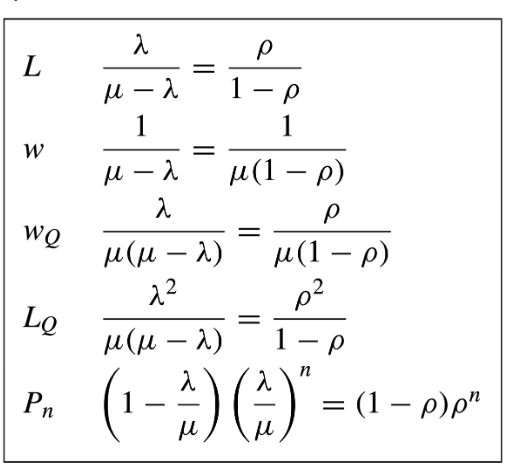
\includegraphics[width=0.5\textwidth]{images/QQ9.png}
    \caption{Infinite population Markovian Models: Case M/M/1}
    \label{fig:student_markov_chain}
\end{figure}